\section{Vergleich verschiedener \textit{Machine Learning}-Algorithmen} \label{sec:compare}
In diesem Kapitel sollen unterschiedliche \textit{Machine Learning}-Algorithmen im Hinblick auf das Projekt miteinander verglichen werden.
Es wurde bereits eine Vorauswahl getroffen und für den Vergleich wurden die Algorithmen \textit{K-Nearest-Neighbor}, die \textit{Support Vector Machine} und
\textit{Convolutional Neural Networks} ausgewählt. Für einen fairen Vergleich wird beim Trainieren aller zuvor genannten \textit{Machine Learning}-Algorithmen
die bereits vorgestellte MNIST-Datenbank verwendet, die Datensätze zu handschriftlichen Ziffern enthält.

Die Kriterien, nach denen der Vergleich durchgeführt werden soll, wurden bereits im Vorfeld definiert. Es wurde sich auf die Kriterien Komplexität,
Präzision, Genauigkeit sowie die Einfachheit der Umsetzung geeinigt. Die \textbf{Komplexität} beschreibt hier die \textit{(Zeit-)}\textbf{Komplexität} des verwendeten Algorithmus und wird mit der O-Notation dargestellt.
Die \textbf{Genauigkeit} bei \textit{Machine Learning}-Algorithmen ist definiert durch die Anzahl der richtig zugewiesenen Trainingsobjekte durch die Anzahl aller
Trainingsobjekte, während die \textbf{Präzision} durch folgende Gleichung bestimmt werden kann:
\[ \text{Präzision} = \frac{\text{Richtig Positiv}}{\text{Richtig Positiv} + \text{Falsch Positiv}} \]
Danach wird die \textbf{Einfachheit der Umsetzung} der zu bewertenden \textit{Machine Learning}-Algorithmen von der testenden Person auf Basis einer Skala von
eins bis fünf beurteilt.

In den folgenden Unterkapiteln werden die drei \textit{Machine Learning}-Algorithmen aus der Vorauswahl näher beschrieben und eine Evaluation nach den genannten 
Kriterien vorgenommen.

\subsection{K-Nearest-Neighbor} \label{ssec:knn}
\textit{[In Bearbeitung durch Dirk Kremer]}


\newpage

\subsection{Support Vector Machine} \label{ssec:svm}
Die \textit{Support Vector Machine} ist ein Algorithmus zur Klassifizierung von Daten in verschiedene Klassen.
Sie wurde in den 1990er Jahren innerhalb der Informatiker-Community entwickelt und gewinnt seitdem immer weiter an Popularität.
\acp{SVM} können in vielen verschiedenen Szenarien eingesetzt werden und werden zu den besten Klassifizierern gezählt.
Bevor die SVM entwickelt wurde, gab es verschiedene Vorgängertechnologien aus denen am Ende die heutige \textit{Support Vector Machine} hervorgegangen ist. 
Diese Algorithmen sind zum Einen der \textit{Maximal Margin Classifier} und der \textit{Support Vector Classifier}, 
der eine Weiterentwicklung des zuvor Genannten darstellt.
Die \textit{Support Vector Machine} ist wiederum eine Erweiterung des \textit{Support Vector Classifier}.
Jeder dieser Klassifizierer wird meist lose unter dem Begriff \textit{Support Vector Machine} zusammengefasst,
müssen jedoch klar unterschieden werden.\cite[S. 337]{james_2013}

Die Terminologie im Bereich der \textit{Support Vector Machine} ist nicht ganz klar und kann sich in verschiedenen Veröffentlichungen unterscheiden.
Eine andere Differenzierung der Vorgängertechnologien ist die Einteilung in Lineare Klassifizierer und nicht-lineare Klassifizierer.
Auch zu erwähnen ist der Lagrangische \textit{Support Vector Machine} Algorithmus, mit dem iterativ SVMs trainiert werden können.\cite[S. 207]{suthaharan_2015}
In dieser Arbeit verwenden wir die zuvor genannte Einteilung in \textit{Maximal Margin Classifier}, \textit{Support Vector Classifier}
und \textit{Support Vector Machine}. An ihr lässt sich die kontinuierliche Weiterentwicklung der Algorithmen am besten verfolgen und am übersichtlichsten darstellen.
Außerdem wird die Chronologie der hinzugekommenen Konzepte deutlicher.

Beginnen wir mit der einfachsten Form dieser Klassifizierer, dem \textit{Maximal Margin Classifier}. 
Dieser wird durch eine sogenannte \textit{Hyperplane} definiert. In einem $p$-dimensionalen Raum ist eine \textit{Hyperplane}
ein flacher affiner Subraum der Dimension $p - 1$. 
Bei zwei Dimensionen wäre eine \textit{Hyperplane} ein flacher $1$-dimensionaler Subraum oder in anderen Worten eine Gerade.
In einem $3$-dimensionalen Raum ist die \textit{Hyperplane} demnach eine Ebene.
\textit{Hyperplanes} in höherdimensionalen Räumen sind schwer für den Menschen vorstellbar, folgen jedoch ebenfalls der Definition.  
Die mathematische Definition einer \textit{Hyperplane} im $2$-dimensionalen Raum lautet:
\[\beta_0 + \beta_1X_1 + \beta_2X_2 = 0\]
mit den Parametern $\beta_0$, $\beta_1$ und $\beta_2$. 
Es lässt sich erkennen, dass die Definition mit der einer Geraden übereinstimmt und damit unserer oben beschriebenen
Definition einer \textit{Hyperplane} folgt.
In einem $p$-dimensionalen Raum wird die Gleichung einer \textit{Hyperplane} wie folgt erweitert:
\[\beta_0 + \beta_1X_1 + \beta_2X_2  + \dots + \beta_pX_p= 0\]
Eine \textit{Hyperplane} teilt den $p$-dimensionalen Raum in zwei Hälften.
Erfüllt ein Punkt $X = (X_1, X_2, \dots, X_p)$ des $p$-dimensionalen Raumes nicht die obige Gleichung,
liegt er entweder auf der einen Seite
\[\beta_0 + \beta_1X_1 + \beta_2X_2  + \dots + \beta_pX_p> 0\]
oder auf der anderen Seite der \textit{Hyperplane}
\[\beta_0 + \beta_1X_1 + \beta_2X_2  + \dots + \beta_pX_p< 0\]
Abbildung \ref{fig:Hyperplane} zeigt beispielhaft eine solche \textit{Hyperplane}, die durch die Gleichung $1 + 6X_1 + 4X_2 = 0$ definiert ist.
Sie trennt den Raum in einen blauen Bereich, wo alle Punkte $1 + 6X_1 + 4X_2 > 0$ erfüllen und eine rote Seite, auf der für alle Punkte $1 + 6X_1 + 4X_2 < 0$ gilt.
\cite[S. 338]{james_2013}
\begin{figure}[H]
	\centering
	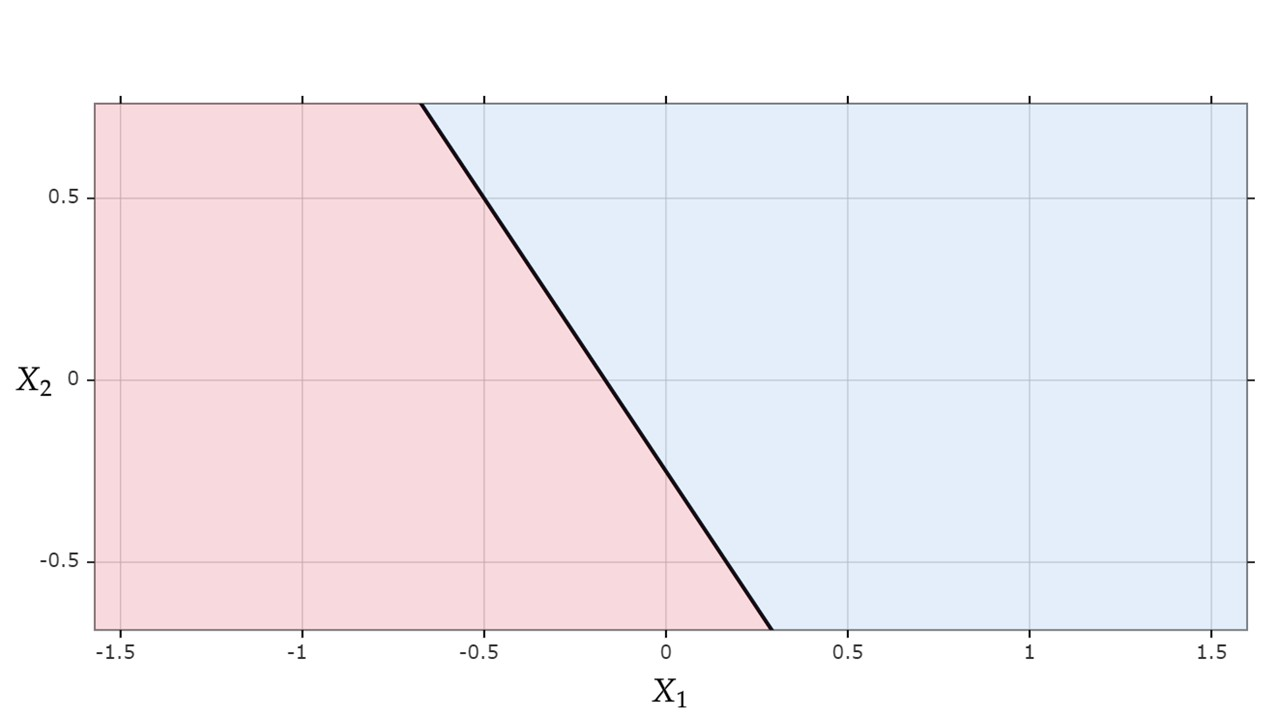
\includegraphics[width=\imgMed]{images/theory/hyperplane.jpg}
	\caption{Beispiel für eine \textit{Hyperplane}} 
	\label{fig:Hyperplane}
\end{figure}
Wir haben nun eine Matrix der Trainingsdaten $\mathbf{X}$ der Form $n \times p$, 
die aus $n$ Trainingsobjekten innerhalb eines $p$-dimensionalen Raumes besteht.
\[x_1 = \left(\begin{array}{c} x_{11} \\ \vdots \\ x_{1p} \end{array}\right) 
  , \dots, 
  x_n = \left(\begin{array}{c} x_{n1} \\ \vdots \\ x_{np} \end{array}\right) \]
Diese Trainingsobjekte sind definiert als Vektoren der Länge $p$, die die einzelnen beobachteten \textit{Features} 
$x^* = (x_1^* \dots x_p^*)^T$ enthalten und werden jeweils einer von zwei Klassen zugeordnet $y_1,\dots,y_n \in \{-1,1\}$.
Wenn die \textit{Hyperplane} die Trainingsobjekte perfekt anhand ihrer Labels trennt,
dann spricht man von einer \textit{separierenden Hyperplane}. 
Alle Objekte aus der einen Klassen fallen auf die linke Seite der \textit{Hyperplane}.
Während die Trainingsobjekte mit dem anderen Label auf der rechten Seite der \textit{Hyperplane} liegen.
Eine \textit{separierende Hyperplane} lässt sich mathematisch definieren durch folgende zwei Gleichungen:
\[\beta_0 + \beta_1X_1 + \beta_2X_2  + \dots + \beta_pX_p> 0 \text{ if } y_i = 1\]
\[\beta_0 + \beta_1X_1 + \beta_2X_2  + \dots + \beta_pX_p< 0 \text{ if } y_i = -1\]
für alle $i = 1 , \dots, n$.
Diese \textit{separierende Hyperplane} kann nun als Klassifizierer eingesetzt werden. 
Um ein unbekanntes Testobjekt nun zu klassifizieren, muss nur geschaut werden auf welcher Seite der \textit{Hyperplane} das Objekt liegt.
Liegt das Testobjekt auf der positiven Seite der \textit{Hyperplane} wird ihm das Label $1$ zugewiesen.
Wenn es auf der negativen Seite liegt, wird das Testobjekt der Klasse $-1$ zugeordnet.
Je weiter entfernt das Testobjekt von der \textit{separierenden Hyperplane} liegt, desto sicherer können wir uns sein,
dass die Klassenzuweisung korrekt ist. Je kleiner der Abstand zur \textit{Hyperplane} wird, desto unsicherer ist,
ob das Testobjekt der richtigen Klasse zugeordnet worden ist. 
Der Abstand der einzelnen Testobjekte zur \textit{separierenden Hyperplane} zeigt uns mit welcher Gewissheit das SVM
die richtige Klassifizierung getroffen hat.\cite[S. 339 - 141]{james_2013}

Beim \textit{Maximal Margin Classifier} wird die oben genannte Methode der \textit{separierenden Hyperplane} eingesetzt,
um Daten klassifizieren zu können. Wenn die Daten durch eine \textit{separierende Hyperplane} getrennt werden können,
gibt es unendlich viele Möglichkeiten, wie diese liegen kann. Für bestmögliche Ergebnisse beim Klassifizieren muss
deshalb die optimale \textit{separierende Hyperplane} gefunden werden. Die natürliche Wahl ist es die 'Mittigste' der
\textit{separierenden Hyperplanes} zu verwenden. Diese wird auch \textit{Maximal Margin Hyperplane} genannt.
Mit Hilfe der Trainingsdaten muss eine \textit{separierende Hyperplane} gefunden werden, die so weit wie möglich von den
nächsten Trainingsobjekten entfernt liegt.\cite[S. 1565f.]{noble_2006}

Die Abbildung \ref{fig:separating_hyperplanes} zeigt zehn verschiedene Trainingsobjekte, die alle durch zwei Variablen definiert sind und
einem der beiden Label $\{blau, rot\}$ zugeordnet sind. Außerdem sind drei unterschiedliche \textit{Hyperplanes} abgebildet, die alle 
\textit{separierende Hyperplanes} im Bezug auf unsere Trainingsdaten sind. Die Auswahl der „perfekten“ \textit{Hyperplane} für die SVM ist
damit ein mathematisches Optimierungsproblem. 
Weitere Informationen zu dem Trainingsmodell einer SVM sind in dem Werk von \citeauthor{suthaharan_2015} zu finden.\cite[S. 210ff.]{suthaharan_2015}
\begin{figure}[H]
	\centering
	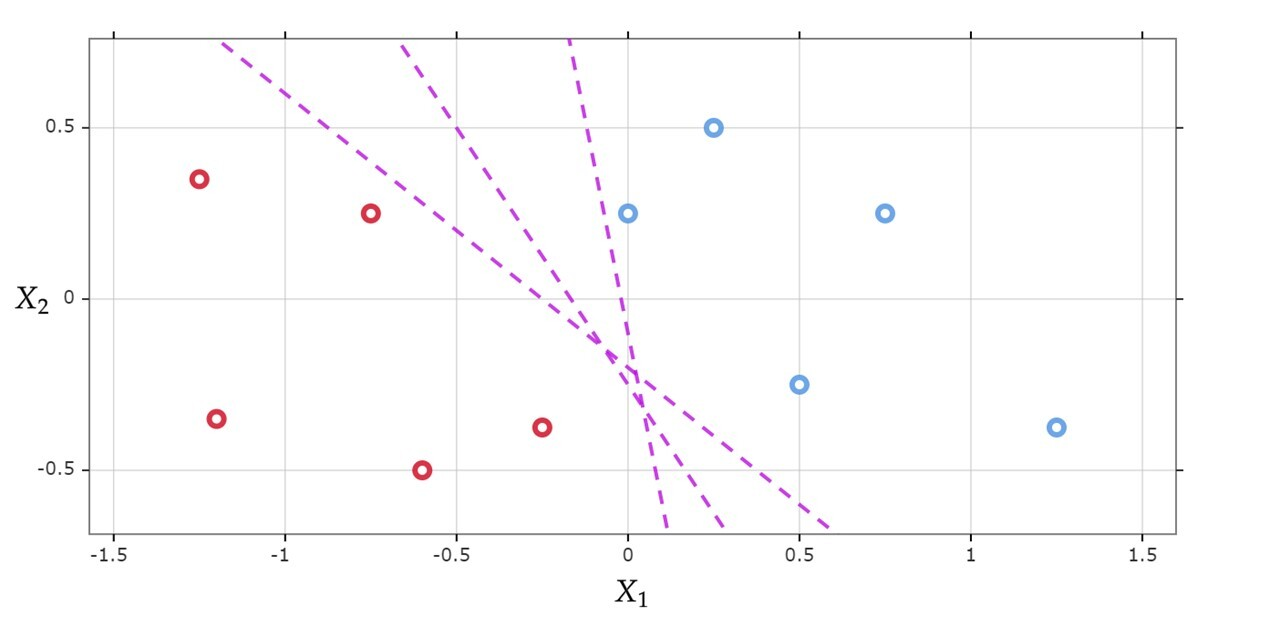
\includegraphics[width=\imgMed]{images/theory/separating_hyperplanes.jpg}
	\caption{Beispiele für \textit{separierende Hyperplanes}} 
	\label{fig:separating_hyperplanes}
\end{figure}
Der Abstand zwischen der \textit{separierenden Hyperplane} und den nächstgelegenen Trainingsobjekten beider Labels
wird als \textit{Margin} bezeichnet. Die \textit{Hyperplane}, deren \textit{Margin} am größten ist,
wird daraus folgend auch \textit{Maximal Margin Hyperplane} genannt.
Die Trainingsobjekte, die am nächsten zu der \textit{Hyperplane} liegen und damit auch denselben Abstand zu dieser haben,
werden als die \textit{Stützvektoren} bezeichnet. Sie „stützen“ die \textit{Maximal Margin Hyperplane}.
Die \textit{Stützvektoren} sind demnach die einzigen Trainingsobjekte, die die Position der \textit{Hyperplane} überhaupt beeinflussen.\cite[S. 341]{james_2013}
Mit Hilfe der \textit{Maximal Margin Hyperplane} kann der 
\textit{Maximal Margin Classifier} nun neue unbekannte Testdaten klassifizieren, je nach dem auf welcher Seite sie liegen.
Je größer dabei die \textit{Margin} der zugrunde liegenden \textit{Hyperplane}, desto erfolgreicher der Klassifizierer.\cite[S. 1566]{noble_2006}

Eine solche \textit{Maximal Margin Hyperplane} ist in \ref{fig:maximal_margin} abgebildet. Die abgebildeten Trainingsdaten sind dieselben
wie auch in Abbildung \ref{fig:separating_hyperplanes}. Es wurde die „mittigste“ \textit{separierende Hyperplane} gefunden, die die Trainingsdaten
anhand ihrer Labels trennen kann. Außerdem zu sehen, sind die am nächsten gelegen Trainingsobjekte auf beiden Seiten der \textit{Hyperplane}, die als
Stützvektoren dienen. Die \textit{Margin} wird visualisiert, durch die beiden Geraden, die parallel zur \textit{separierenden Hyperplane} liegen und
durch die beiden \textit{Stützvektoren} verlaufen. Der Abstand dieser beiden Geraden zu der \textit{Hyperplane} ist die \textit{Margin}.
\begin{figure}[H]
	\centering
	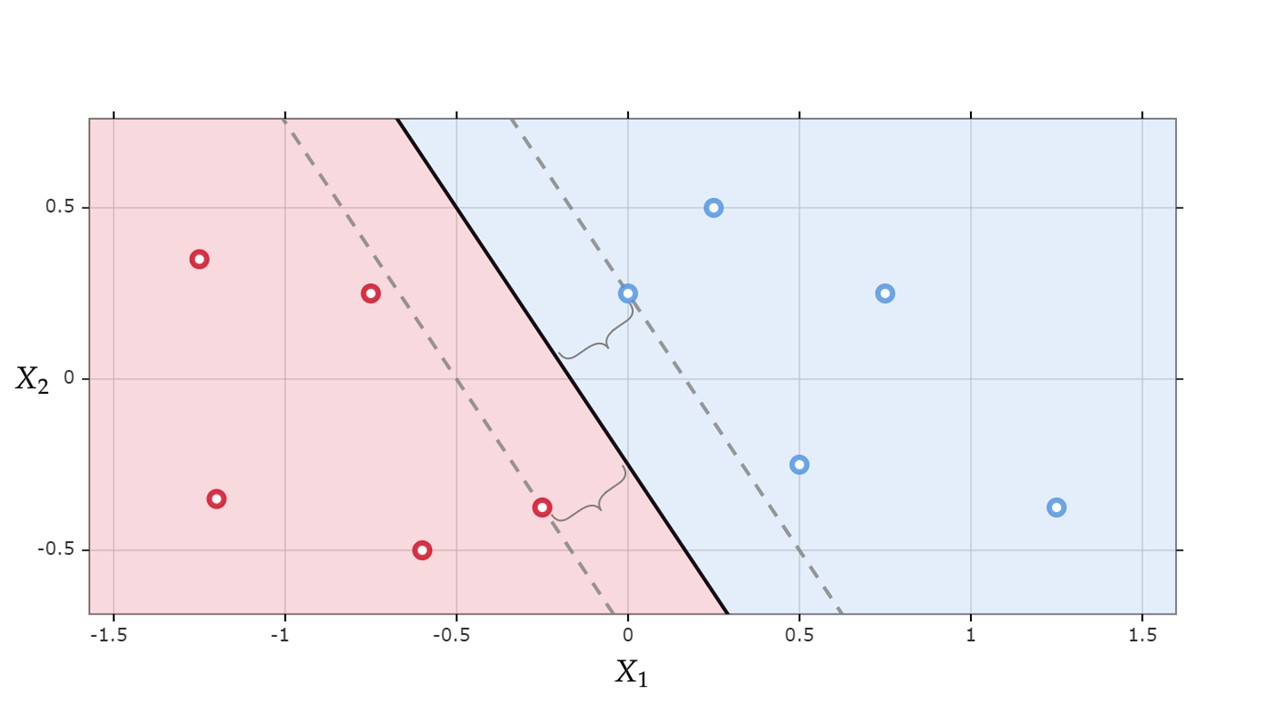
\includegraphics[width=\imgMed]{images/theory/maximal_margin.jpg}
	\caption{Beispiel für eine \textit{Maximal Margin Hyperplane}} 
	\label{fig:maximal_margin}
\end{figure}
Je nach Trainingsdaten gibt es Szenarien in denen keine \textit{separierende Hyperplane} existiert, die die Daten perfekt anhand ihrer Labels
trennen kann oder die \textit{Hyperplane} liegt nicht optimal, um eine effiziente Klassifizierung durchführen zu können, da die
textit{Stützvektoren} ungünstig liegen. Der \textit{Maximal Margin Classifier} hat eine hohe Sensibilität für einzelne Trainingsobjekte
und kann demnach leicht übertrainiert werden. Es können zum Beispiel Trainingsobjekte existieren deren \textit{Features} nicht den Normen einer Klasse entsprechen 
und damit eine Anomalie darstellen. Das besagte Trainingsobjekt würde dann auf der falschen Seite der zuvor gefundenen \textit{Hyperplane} liegen.
Deswegen müssen, um eine bessere Klassifizierung und eine höhere Robustheit für einzelne Trainingsobjekte
zu gewährleisten, auch nicht perfekt \textit{separierende Hyperplanes} in Betracht gezogen werden.\cite[S. 343 - 345]{james_2013}

Dies wird vom \textit{Support Vector Classifier} umgesetzt. Er wird auch als \textit{Soft Margin Classifier} bezeichnet.
Wie der Name schon sagt, besitzt dieser eine 'weiche' \textit{Margin}. 
Der \textit{Support Vector Classifier} erweitert den bereits besprochenen \textit{Maximal Margin Classifier}
um eine 'weiche' \textit{Margin}, die von einem Nutzer-definierten Parameter abhängig ist.
Der Nutzer muss selbst entscheiden, wie durchlässig die \textit{Margin} sein soll und
wie vielen Trainingsobjekten erlaubt werden soll die \textit{Margin} zu durchdringen, ohne deren finale Ausrichtung zu beeinflussen.
Wie dieser Parameter gesetzt werden muss, hängt von den Trainingsdaten und dem gewünschten Ergebnis ab
und muss durch Ausprobieren ermittelt werden.
Beim Setzen dieses Parameters muss zwischen Durchlässigkeit der \textit{Hyperplane} und der Breite der \textit{Margin} abgewägt werden.
Durch diese 'weiche' \textit{Margin} werden vereinzelt Testobjekte mit anormalen Charakteristiken der falschen Klasse
zugeordnet. Für die meisten Testobjekte steigt jedoch die Genauigkeit der Klassifizierung und aufgrund der 'weichen' \textit{Margin}
ist es leichter eine \textit{separierende Hyperplane} zu finden.\cite[S. 1566]{noble_2006}

Trotzdem gibt es immer noch Szenarien bei denen die Trainingsdaten nicht durch einen \textit{Support Vector Classifier} getrennt
werden können. In manchen Fällen sind die Trainingsdaten nicht linear zu trennen.
In diesen Fällen muss der \textit{Feature}-Raum erweitert werden. Hierfür wurde aus dem \textit{Support Vector Classifier}
die \textit{Support Vector Machine} entwickelt. Dabei wurden sogenannte \textit{Kernel}-Funktionen hinzugefügt.
Mit Hilfe von quadratischen, kubischen oder weiteren Polynomfunktionen höherer Grade wird der \textit{Feature}-Raum der
Trainingsobjekte erweitert. Auf Basis der bisherigen \textit{Features} werden so mathematisch neue \textit{Features} berechnet, die 
dann womöglich durch eine \textit{Hyperplane} zu trennen sind, jedoch von den ursprünglichen \textit{Features} abhängig sind.
Der \textit{Feature}-Raum wird so gesehen von den \textit{Kernel}-Funktionen um eine oder mehrere Dimensionen erweitert.
Auch bei diesen \textit{Kernel}-Funktionen gibt es keine genaue Regel und die für die Trainingsdaten passende 
\textit{Kernel}-Funktion muss durch Ausprobieren gefunden werden. So können nun auch nicht-lineare Daten klassifiziert werden.
\cite[S. 1566f.]{noble_2006}\cite[S. 224 - 227]{suthaharan_2015}

Die nachfolgende Abbildung \ref{fig:non_linear_data} zeigt zwei Beispiele hypothetischer Trainingsdaten, die nicht linear zu trennen sind.
Der \textit{Feature}-Raum wurde mit Hilfe einer \textit{Kernel}-Funktion erweitert und es konnte in einem höherdimensionalen Raum eine
\textit{separierende Hyperplane} gefunden werden, die die Trainingsobjekte anhand ihrer Labels trennen kann. 
Die zwei Grafiken zeigen nun wie diese höherdimensionale \textit{Hyperplane} in einem $2$-dimensionalen Raum aussehen würde 
und wie sie die Daten anhand ihrer Klasse aufteilt.
\begin{figure}[H]
	\centering
	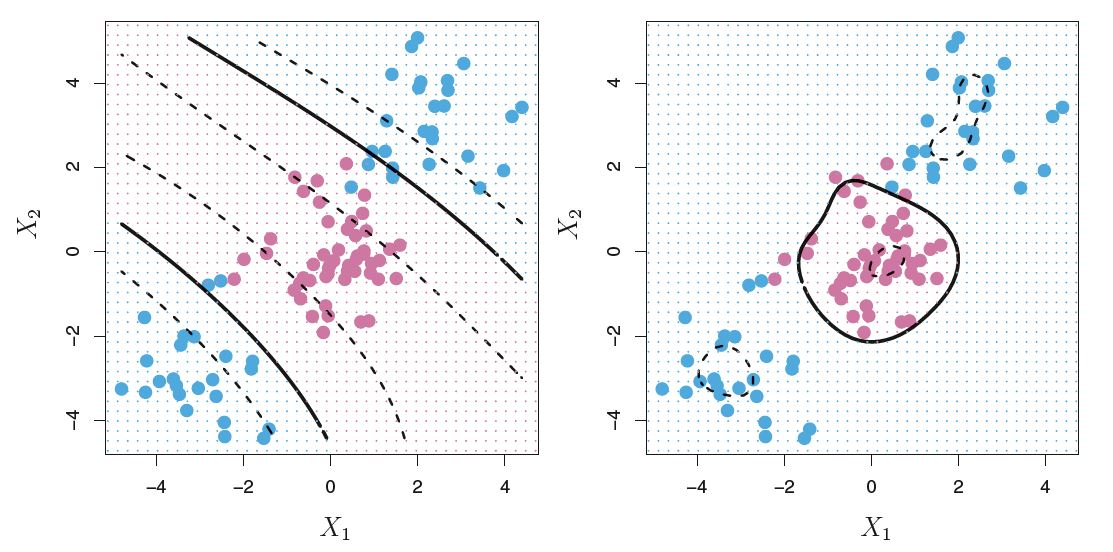
\includegraphics[width=\imgMed]{images/theory/non_linear_data.jpg}
	\caption{\textit{Hyperplanes} bei nicht-linearen Daten \cite[S. 353]{james_2013}} 
	\label{fig:non_linear_data}
\end{figure}
Mit Hilfe der \textit{Support Vector Machine} können wir nun einen Großteil an Datensätzen klassifizieren. 
Eine \textit{separierende Hyperplane} kann die Trainingsdaten jedoch immer nur in zwei Klassen einteilen. 
Wie können dann handgeschriebene Ziffern und Zahlen durch eine \textit{Support Vector Machine} erkannt werden?
Es gibt zwei Möglichkeiten dies zu bewerkstelligen, wenn $K > 2$ Klassen existieren.
Die erste Methode ist die 1-gegen-1-Klassifizierung. Hier wird für jede Paarung der Klassen $K \choose 2$ eine SVM erzeugt. Bei einer Klassifizierung eines neuen Testobjektes wird die Klasse ausgewählt, zu der das Objekt bei den
$K \choose 2$ paarweisen Klassifizierern am häufigsten zugewiesen wurde.
Die Alternative zu dieser Methode ist die 1-gegen-alle-Klassifizierung. Hier werden $K$ SVMs erstellt.
Eine SVM für jede Klasse und die $K-1$ restlichen Klassen. Ein unbekanntes Testobjekt wird dann der Klasse zugeordnet,
bei der die SVM sich am sichersten bei der Zuordnung ist. 
So kann die \textit{Support Vector Machine} auch Testobjekte verschiedener Klassen unterscheiden.\cite[S. 355f.]{james_2013}\cite[S.1567]{noble_2006}

\subsubsection{Bewertung der \textit{Support Vector Machine}}
Für einen fairen Vergleich zwischen den einzelnen \textit{Machine Learning}-Algorithmen muss die \textit{Support Vector Machine}
nach den bereits festgelegten Bewertungskriterien: Komplexität, Genauigkeit, Präzision und Einfachheit der Umsetzung beurteilt werden.
Die mathematische Komplexität des \textit{Support Vector Machine}-Algorithmus lässt sich nachschlagen.
Das Trainieren einer SVM hat eine Komplexität von $O(n^2 p + n^3)$ mit $n$ als Anzahl der Traingsobjekte und $p$ als Anzahl der \textit{Features}.
Bei dieser Komplexität wird angenommen, dass die \textit{Support Vector Machine} eine \textit{Kernel}-Funktion $K(x_i, x_j)$ besitzt.
Davon ausgehend, dass die häufigsten \textit{Kernel}-Funktionen eine Komplexität von $O(p)$ besitzen, können wir auf die obige Komplexität
für die SVM schließen. Das ist bei Gaußschen, Polynom- und Sigmoidfunktionen der Fall, muss jedoch nicht für jede \textit{Kernel}-Funktion gelten.
Die Komplexität bei dem Klassifizieren der Testdaten entspricht dann $O(n_{sv} p)$. Hier ist $n_{sv}$ die Anzahl der Stützvektoren.\cite{complexity}

Um die Genauigkeit und Präzision einer \textit{Support Vector Machine} bewerten zu können, soll ein kurzes Testprogramm geschrieben werden.
Hierfür wurde die Programmiersprache \textbf{Python} verwendet, die mit \textbf{SciKit-learn} bereits eine Bibliothek für die Anwendung 
verschiedener \textit{Machine Learning}-Algorithmen besitzt. Das fertige Programm ist in \ref{lst:test_svm} zu sehen.
Zuerst werden die benötigten Funktionen aus der \textbf{SciKit-learn}-Bibliothek importiert. Dann wird der 1797-große Datensatz geladen, der die
geschriebenen Ziffern $0, \dots 9$ enthält und die Daten mit Hilfe eines \textbf{NumPy}-\textit{Arrays} vorbereitet. Danach werden die Daten halbiert und in einen
Trainingsdatensatz, sowie in einen Testdatensatz aufgeteilt. Mit \textbf{SciKit-learn} lässt sich dann in zwei Zeilen ein SVM-Objekt erstellen und
mit dem Trainingsdatensatz trainieren. Danach werden die Testdaten in die SVM gegeben und am Ende in einem Klassifizierungsbericht ausgewertet.

\begin{minipage}{\textwidth}
	\begin{lstlisting}[language=Python, caption=Pythoncode zum Testen der SVM, label=lst:test_svm]
# Importieren relevanter Bibliotheken
from sklearn import svm
from sklearn import metrics
from sklearn.datasets import load_digits
from sklearn.model_selection import train_test_split

# Laden des SciKit-learn-Datensatzes
digits = load_digits()

# Vorbereiten der Daten
n_samples = len(digits.images)
data = digits.images.reshape((n_samples, -1))

# Aufteilen der Daten in Trainings- & Testdaten
X_train, X_test, y_train, y_test = train_test_split(
    data, digits.target, test_size=0.5, shuffle=False)

# Trainieren der SVM mit den Trainigsdaten
svm_classifier = svm.SVC(gamma=0.001)
svm_classifier.fit(X_train, y_train)

# Klassifizieren der Testdaten
predicted = svm_classifier.predict(X_test)

# Ausgeben der Ergebnisse
print("\nKlassifizierungsbericht %s:\n%s\n" % (svm_classifier, metrics.classification_report(y_test, predicted)))
print("\nGenauigkeit: ", svm_classifier.score(X_test, y_test))
	\end{lstlisting}
\end{minipage}

Aus dem Klassifizierungsbericht in \ref{lst:testergebnis_svm} kann direkt die Präzision und Genauigkeit dieser \textit{Support Vector Machine} 
herausgelesen werden. Die \textit{Support Vector Machine} aus unserem Test hat eine durchschnittliche Präzision von $0.97$, sowie eine 
gerundete Genauigkeit von ebenfalls $0.97$.

\begin{minipage}{\textwidth}
	\begin{lstlisting}[language=Bash, caption=Testergebnisse der SVM, label=lst:testergebnis_svm]
Klassifizierungsbericht SVC(gamma=0.001):
			   precision    recall  f1-score   support

		0         1.00      0.99      0.99        88
		1         0.99      0.97      0.98        91
		2         0.99      0.99      0.99        86
		3         0.98      0.87      0.92        91
		4         0.99      0.96      0.97        92
		5         0.95      0.97      0.96        91
		6         0.99      0.99      0.99        91
		7         0.96      0.99      0.97        89
		8         0.94      1.00      0.97        88
		9         0.93      0.98      0.95        92

accuracy                          0.97       899
macro avg    	0.97      0.97      0.97       899
weighted avg 	0.97      0.97      0.97       899

Genauigkeit:  0.9688542825361512
	\end{lstlisting}
\end{minipage}

Damit ist bereits eine Mehrheit der Kriterien zur Bewertung der SVM abgedeckt. Als Letztes muss nun die Einfachheit der Umsetzung bewertet werden.
Es spricht für die \textit{Support Vector Machine}, dass uns die gesamte Umsetzung des Algorithmus bereits abgenommen wurde und alle benötigten
Funktionen durch die \textbf{Python}-Bibliothek \textbf{SciKit-learn} bereitgestellt wurden. Die \textit{Support Vector Machine} ist damit sehr einfach
für unser Projekt zu verwenden.  Wie bereits im obigen Beispielcode \ref{lst:test_svm} zu sehen, braucht es nur drei Zeilen Code um eine SVM zu initialisieren,
zu trainieren und neue Testdaten zu klassifizieren. Deshalb gebe ich der \textit{Support Vector Machine} eine Punktzahl von 5/5.
Damit ist die Bewertung der dieses \textit{Machine Learning}-Algorithmus abgeschlossen. 
Als Nächstes folgt eine Erläuterung der \textit{Convolutional Neural Networks} und deren Beurteilung.

\newpage

\subsection{Convolutional Neural Networks} \label{ssec:cnn}
Die letzte künstliche Intelligenz, die es in diesem Vergleich zu untersuchen gilt, ist die des \acp{CNN}.

Die CNN wird, ähnlich wie die SVM als ein Konstrukt zum Klassifizieren von Bildern genutzt, jedoch unterscheiden sie sich in der Herangehensweise das Problem zu lösen. Anders als die SVM handelt es sich bei der CNN um keine algorithmische Umsetzung, sondern um eine vordefinierte Menge an Anweisungen, die zur Lösung eines spezifischen Problems führen. Aufgrund der vordefinierten Menge an Anweisungen ist ein CNN jedoch auf Probleme beschränkt, welche wir verstehen und lösen können. Dies hat zur Folge, dass kein Ansatz dem anderen überzuordnen ist, sondern die Art des Problems definiert, ob konventionelle Algorithmen oder neuronale Netzwerke besser geeignet sind. \cite*{10.1007/978-3-319-45378-1_1}

Um nun den Aufbau eines CNN zu verstehen, betrachten wir zunächst ein normales \ac{ANN} oder \textit{Neural Network}. Beide Terminologien werden in der Literatur kommutativ genutzt. Um den Unterschied zu den biologischen neuronalen Netzwerken zu verdeutlichen, wird fortlaufend in dieser Arbeit ANN als Terminologie genutzt.

\subsubsection{Artificial Neural Network}
Im Jahr 1943 entwickelte der Neurophysiologe Warren McCulloch und ein junger Mathematiker Walter Pitts das erste Model eines ANN, das in der Studie „The Logical Calculus of the Ideas Immenent in Neverous Activiy“ veröffentlicht wurde. Dieses war in der Lage, einfache logische Operationen durchzuführen.
Im Laufe der Historie wurde das Konstrukt ANN immer weiterentwickelt und hat in der Informatiker-Community an Ansehen erlangt, bis die Technologie an ihre damaligen Grenzen gestoßen ist und die Technologie zunächst vernachlässigt wurde.
Heutzutage sind ANN einer der wichtigsten Bestandteile in der Erforschung der Künstlichen Intelligenz und des maschinellen Lernens, welches auf die enorme Innovation in der Computerindustrie und der Leistungsverbesserung der Rechner zurückzuführen ist. \cite*{10.1007/978-3-319-45378-1_1}

Ein ANN ist im Aufbau ähnlich zu einem primitiven biologischen Nervensystem. Es besteht aus einer gewissen Anzahl an Knoten, die Neuronen repräsentieren und miteinander verbunden sind. Die miteinander verbunden Knoten geben Informationen an den jeweils nächsten Knoten weiter, nachdem ihre eingegangene Information verarbeitet wurde.
In einem ANN sind die Knoten in verschiedene Schichten aufgeteilt, wobei die Anzahl der Knoten nicht festgelegt ist. Es können Schichten mit einem Knoten erstellt werden oder mit mehreren Tausenden. Jede dieser Schichten dient einem genau definierten Zweck im Netzwerk. Um den Zweck genauer zu definieren, werden die Schichten in drei Gattungen unterteilt, in die Eingabeschicht, die versteckten Schichten und die Ausgabeschicht. Die Eingabeschicht nimmt in der Regel einen mehrdimensionalen Eingabevektor entgegen. Dieser wird in der Eingabeschicht verarbeitet und das Ergebnis wird an die Knoten der nächsten Schicht verteilt. Die danach kommende Schicht verarbeitet die Informationen, die sie bekommen hat und verteilt diese dann wieder an die nächsten Knoten in der folgenden versteckten Schicht oder an die Ausgabeschicht, wenn keine weitere verdeckte Schicht folgt.
Die Knoten innerhalb einer Schicht sind nicht miteinander verknüpft, sie sind nur mit Knoten aus der vorherigen und danach kommenden Schicht verbunden. Wenn alle Knoten mit allen Konten aus der vorangegangen und danach kommenden Schicht verbunden sind, bezeichnet man das ANN an diesem Punkt als \textit{fully-connected}. Ein solches \textit{fully-connected ANN} ist in Abbildung \ref{fig:ful_con_ann} zu erkennen. Das Netzwerk verfügt beispielsweise über vier Schichten, eine Eingabeschicht, eine Ausgabeschicht und zwei versteckten Schichten. In der Abbildung werden die Knoten als Kreise dargestellt und die Verbindungen als gerichtete Linien. Die versteckten Schichten haben zum Beispiel vier Knoten.
\cite*{Keiron2015}

\begin{figure}[H]
	\centering
	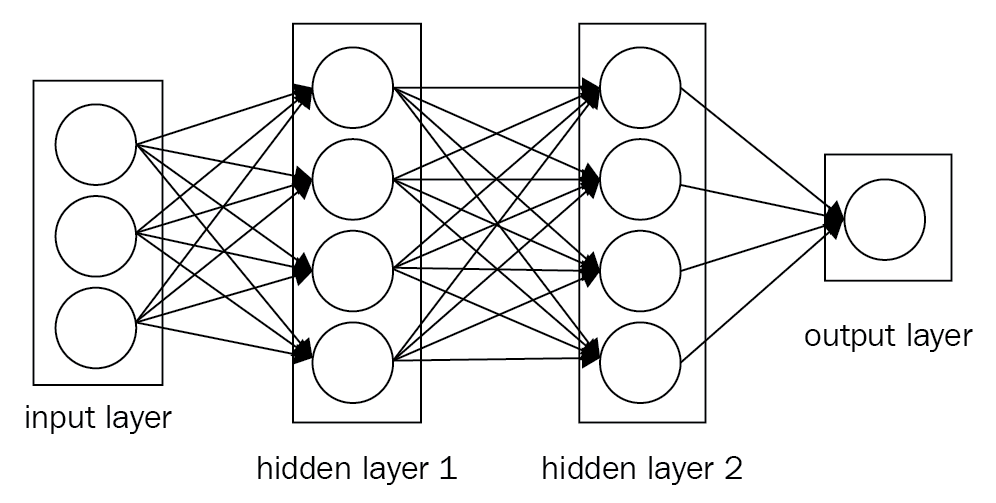
\includegraphics[width=\imgMed]{images/theory/neural_network.png}
	\caption{Ein \textit{fully-connected ANN} mit zwei versteckten Schichten \cite{Sewak2018}} 
	\label{fig:ful_con_ann}
\end{figure}

Um nun genauer nachzuvollziehen, wie ein Knoten in einem ANN operiert, gehen wir genauer auf die mathematische Definition eines Knotens ein. \\    
Die Verarbeitung der Eingabevektoren erfolgt durch die Anwendung der sogenannten Aktivierungsfunktion $a$. Die Aktivierungsfunktion ist die Summe der gesamten Eingabevektoren $[x_1,…,x_n]$ multipliziert mit einer Gewichtsmatrix $[w_1,...,w_n]^T$,
wobei \textit{n} die Anzahl der vorherigen Knoten ist. Mathematisch ist sie wie folgt definiert:

\[a = \sum_{i=1}^{n} x_i w_i\]

In der Abbildung \ref{fig:act_fun} wird die Aktivierungsfunktion $a$ dargestellt. Es ist erkennbar, wie jeder Eingabevektor $x_i$ mit einem Gewicht $w_i$ multipliziert wird und anschließend die Summe aller Ergebnisse gebildet wird. Das Ergebnis der Aktivierungsfunktion $a$ ist die Ausgabe eines Knotens und wird anschließend von den folgenden Knoten in der nächsten Schicht als Eingabevektor verarbeitet. 

\begin{figure}[H]
	\centering
	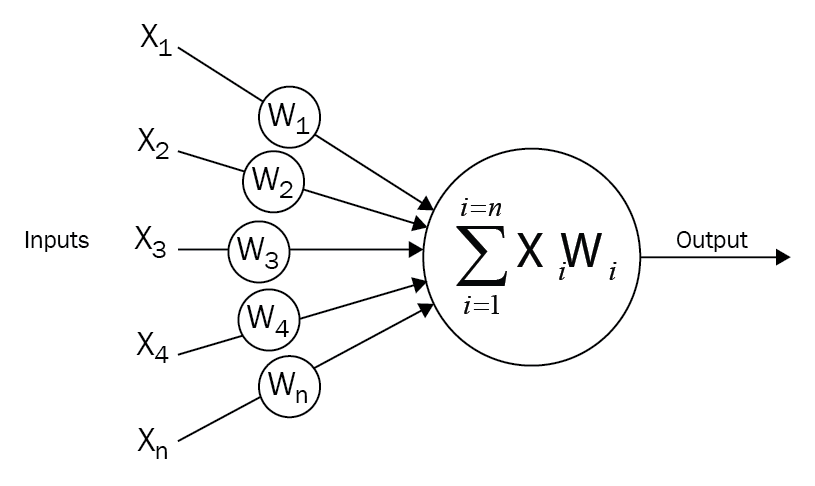
\includegraphics[width=\imgMed]{images/theory/activationfunction.png}
	\caption{Bildliche Darstellung der \textit{Aktivierungsfunktion} \cite{Sewak2018}} 
	\label{fig:act_fun}
\end{figure}

Mit dieser Funktion können wir nachvollziehen, wie jeder einzelne Knoten seine Entscheidung trifft.\cite*{Braspenning1995}

Zusätzlich können wir eine \textit{Verlustfunktion} für das Netzwerk definieren, um die Genauigkeit der Entscheidungen zu messen. Bei den ANN existieren zwei verschiedene Arten von Verlustfunktionen, die Klassifizierungs-Verlustfunktion und die Regression-Verlustfunktion. 
Die Klassifizierung-Verlustfunktion wird genutzt, wenn ein Netzwerk als Klassifizierer eingesetzt wird, wie es in diesem Test der Fall ist. Die Regression-Verlustfunktion wird bei Anwendungen der Vorhersage von bestimmten Werten verwendet.
Unter den zwei Arten der Verlustfunktion für ANN existieren wiederum verschiedene mathematische Funktionen, mit denen sich der Wert je nach Anwendung berechnen lässt.\cite{dwivedi_2020}

Im Folgenden wird die sogenannte \textit{Kreuzentropie} oder auch \textit{log-loss} genannt als Verlustfunktion verwendet. Diese Verlustfunktion wird bei binärer Klassifikation eingesetzt und berechnet den Verlustwert mit Hilfe eines booleschen Wertes und dem errechneten Entscheidungswert des ANN. Der boolesche Wert wird durch 0 oder 1 ausgedrückt, dieser sagt aus, ob das zu klassifizierende Objekt richtig erkannt wurde oder nicht. In der Abbildung \ref*{fig:crossentropy} wird die Kreuzentropie dargestellt. Anhand dieser Darstellung ist zu erkennen, wie der Verlustwert abhängig vom Entscheidungswert des ANN ist. Wenn der Entscheidungswert sich der 1 annähert, verringert sich der Wert der Kreuzentropie.
Für eine Klassifikation von zwei Klassen wird die Kreuzentropie wie folgt berechnet: 

\[-(y\times log(p) + (1 - y) \times log(1-p))\]

\begin{itemize}
	\item $y$ ist der boolesche Wert, der angibt, ob das zu klassifizierende Objekt richtig erkannt wurde.
	\item $p$ ist der errechnete Entscheidungswert des ANN.
\end{itemize}

Im Fall der Zahlenerkennung existiert für jede Zahl eine Klasse. Das Prinzip der Kreuzentropie lässt sich auf eine beliebige Anzahl von Klassen erweitern, in dem für jedes Label pro Beobachtung der Verlustwert berechnet wird und letztendlich summiert wird.

\[ -\sum_{c=1}^{M}y_{o,c} \times log(p_{o,c}) \]

\begin{itemize}
	\item $c$ ist das Klassenlabel.
\end{itemize}
\cite{10.2307/2348828}

\begin{figure}[H]
	\centering
	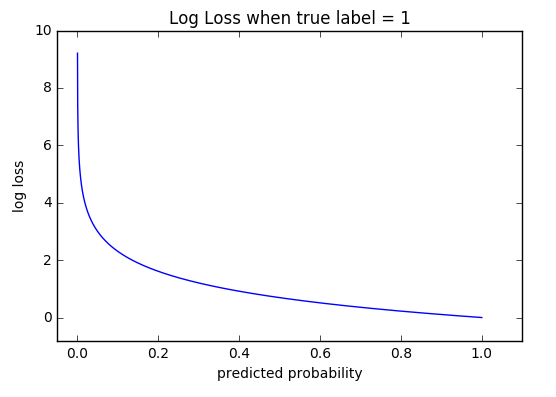
\includegraphics[width=\imgMed]{images/theory/cross_entropy.png}
	\caption{Graph einer \textit{Kreuzentropie} \cite{fortuna_viana_2019}} 
	\label{fig:crossentropy}
\end{figure}

\subsubsection*{Von Artificial Neural Network zu Convolutional Neural Network}
Wie im Vorfeld angeführt, handelt es sich bei den CNN um eine Spezialisierung eines ANN. Diese Spezialisierung erweitert und spezifiziert Aspekte eines ANNs, welche im Folgenden genauer erläutert werden.

Da wir das CNN für die Klassifikation von Bildinhalten verwenden, muss die Eingabeschicht für diesen Datentypen vorbereitet werden. Die Besonderheit hierbei liegt darin, dass die Knoten zusätzlich zu den Schichten in drei Dimensionen aufgeteilt werden. Diese Aufteilung bezieht sich jedoch nur auf die Verknüpfungen zu den Knoten in der nächsten Schicht. Die Dimensionen sind für ein Bild die Höhe und Breite. Eine zusätzliche dritte Dimension ist die sogenannte Tiefe, welche Auskunft über die Anzahl der folgenden verknüpften Knoten bietet.

Die Architektur der CNN erweitert das Prinzip der Ein/Ausgabeschicht und den versteckten Schichten insoweit, als dass die versteckten Schichten in weitere Kategorien eingeteilt werden können. Bei einem CNN gibt es zusätzlich zu der Ein/Ausgabeschicht, die Filter-Schichten (engl. Convolutional Layer), Aggregations-Schichten (Pooling Layer) und die vollständig verbundenen Schichten (engl. Fully Connected Layer, Dense Layer).
Bei der Ausgabeschicht handelt es sich ebenfalls um eine vollständig verbundene Schicht. \cite*{Keiron2015}

Die einzelnen Aufgaben und Eigenarten der verschiedenen Schichten werden im Folgenden behandelt.

\subsubsection{Input Layer}
In der Eingabeschicht werden die Bilddaten gespeichert und in einer dreidimensionalen Matrix dargestellt.\cite*{Sewak2018}

\subsubsection{Filter-Schicht}
Die Filter-Schicht, auch häufig als Feature-Extraction-Layer bezeichnet, extrahiert Eigenschaften aus dem Eingabebild und übt die Hauptanzahl an Berechnungen aus. 
Es handelt sich hierbei um Faltungsoperationen, die Ähnlichkeiten zur Fourier-Transformation und zur Lapace-Transformation aufweisen, und bilden das Merkmal eines CNNs.
Ein Neuron einer Filter-Schicht betrachtet einen bestimmten Bereich einer vorherigen Schicht in Form einer Matrix und bildet daraus ein Skalarprodukt, um die den Bereich auf nur eine Zahl zu reduzieren.
Die Architektur eines CNNs, die aus den verschiedenen Schichten und der Filter-Schichten besteht, ermöglichen, dass weniger Neuronen benötigt werden im Gegensatz zu anderen vielschichtigen neuronalen Netzwerken.\cite*{Sewak2018}
Die Knoten in der Filter-Schicht nutzen die sogenannte \ac{ReLU}-Funktion als Aktivierungsfunktion. Diese ist, wie der Name bereits beschreibt, eine lineare Funktion, welche leicht modifiziert ist, sodass der Rückgabewert der Funktion gleich null ist, wenn der Eingabewert kleiner gleich null ist. Das bringt diverse Vorteile bei der Optimierung von CNNs und ANNs. Lineare Funktionen sind leichter zu optimieren und zu trainieren. Die ReLU Funktion lässt sich mathematisch als das Maximum einer Menge definieren, welche zwei Elemente besitzt, den Wert $0$ und den Wert $x$.

\[ReLU(x) = max\{0, x\}\] \cite*{goodfellow2016}

\subsubsection{Aggregations-Schicht}
Die Aggregations-Schicht ist für das Heruntertasten der Dimensionen zuständig, um die Parameter der Aktivierungsfunktion zu reduzieren. Durch die Anwendung der zuvor liegenden Filter-Schichten wird die räumlichen Dimension erhöht und die damit einhergehend Anzahl der Parameter der darauf folgenden Schicht. Dies hat zur Folge, dass die Komplexität des Models erhöht wird. Diese Überanpassung wird mit den Aggregations-Schichten entgegengewirkt.\cite*{Sewak2018}
Für das Skalieren wird am häufigsten die \textit{max pooling} Funktion verwendet. Diese Funktion reduziert die Dimensionen, ausgenommen der Tiefe, auf eine Größe von etwa 25\% der Originalgröße.\cite*{Keiron2015}

\subsubsection{Vollständig-Verbundene-Schicht}

Die vollständig verbundene Schicht ist die einer versteckten Schicht in einem ANN gleich. Diese Schicht ist hauptsächlich für die Klassifizierung und Berechnungen der Wahrscheinlichkeit zuständig. Die Aktivierungsfunktion der Knoten in dieser Schicht ist wie bei der Filter-Schichten die ReLU Funktion.
Einleitet wurde erwähnt, dass es sich bei der Ausgabeschicht ebenfalls um eine vollständig verbundene Schicht handelt. Diese wird auch als \textit{soft-max} Schicht bezeichnet und gibt die letztendliche Klassifizierung des Bildes zurück.\cite*{Sewak2018}

\newpage

\subsubsection{Bewertung ded Convolutional Neural Networks}

Damit wir ein CNN mit der SVM und dem KNN vergleichen können, werden dieselben Bewertungskriterien untersucht. Die für die Bewertung relevanten Kriterien waren:

\begin{itemize}
\item Komplexität
\item Genauigkeit
\item Präzision
\item Einfachheit der Umsetzung
\end{itemize}

Bevor wir genauer auf die Bewertungskriterien eingehen, werden wir uns mit dem für den Test konstruierten CNN beschäftigen.
Dieser wurde in der Programmiersprache \textbf{Python} Version 3.9 geschrieben. Für die Konstruktion und die Ausführung des Tests benötigen wir verschiedene Bibliotheken, die dabei helfen können, die Bewertungskriterien zu ermitteln, sowie den CNN zu modellieren. Bei diesem Test wurde die Bibliothek \textbf{Tensorflow} verwendet, welche wiederum die \textbf{Keras} Bibliothek verwendet. Zusätzlich wurde die Bibliothek \textbf{NumPy} und \textbf{matplotlib} verwendet, um mit Hilfe von \textit{NumPy} die Daten zu strukturieren und mit \textit{matplotlib} die Ergebnisse darzustellen. Den Programmcode zum Importieren der notwendigen Bibliotheken, sowie die Vorbereitung für den CNN ist in Codeabschnitt \ref{lst:test_prep_cnn} zu finden. In diesem Abschnitt werden zunächst die Bibliotheken importiert und die MNIST-Datenbank wird geladen. Beim Laden der Daten werden die Daten bereits in Trainingsobjekte und Testobjekte unterteilt.

\begin{minipage}{\textwidth}
	\begin{lstlisting}[language=Python, caption=Pythoncode zur Testvorbereitung vom CNN, label=lst:test_prep_cnn]
import tensorflow as tf
import numpy as np
import matplotlib.pyplot as plt
from keras import backend as K

mnist = tf.keras.datasets.mnist

(x_train, y_train), (x_test, y_test) = mnist.load_data()

y_train = y_train.astype('float32')
y_test = y_test.astype('float32')

# Erstellung von Binaerendaten 
mask = x_train > 127.5
maskb = x_train <= 127.5
x_train[mask] = 255
x_train[maskb] = 0

# Shift to -1 to 1
x_train, x_test = (x_train - 127.5) / 127.5, (x_test - 127.5) / 127.5

# Datenaufteilung fuer Validierung
x_val = x_train[-10000:]
y_val = y_train[-10000:]
x_train = x_train[:-10000]
y_train = y_train[:-10000]

	\end{lstlisting}
\end{minipage}

Im folgenden Codeabschnitt wird das CNN-Model definiert. Das Model wurde mit folgenden Schichten definiert:

\begin{itemize}
	\item Filter-Schicht (Eingabeschicht)
	\item Filter-Schicht
	\item Filter-Schicht
	\item Aggregations-Schicht
	\item Vollständig-verbundene-Schicht
	\item Vollständig-verbundene-Schicht (Ausgabeschicht)
\end{itemize}

Die zusätzlich zu sehenden Schichten \textit{Dropout} und \textit{Flatten} wurden definiert, um die Komplexität des Models zu reduzieren. Dieser Effekt ist nur während des Trainierens sichtbar. Bei der \textit{Dropout}-Schicht handelt es sich um eine Schicht, die mit einer gewählten Wahrscheinlichkeit von \textit{0,25} einen Knoten aus der Schicht ausschaltet, um \textit{overfitting} zu verhindern. Die \textit{Flatten}-Schicht formt die mehrdimensionalen Daten in eine einzelne Dimension um, damit diese von der vollständig-verbunden-Schicht verarbeitet werden kann.

\begin{minipage}{\textwidth}
	\begin{lstlisting}[language=Python, caption=Pythoncode zur Konstuktion vom CNN, label=lst:test_cnn]
#CNN
model = tf.keras.models.Sequential([
		tf.keras.layers.Conv2D(32, kernel_size=(3, 3),
							activation='relu',
							input_shape=(28, 28, 1)),
	tf.keras.layers.Conv2D(32, kernel_size=(3, 3),
							activation='relu'),
	tf.keras.layers.Conv2D(32, kernel_size=(3, 3),
							activation='relu'),
	tf.keras.layers.MaxPooling2D(pool_size=(2, 2)),
	tf.keras.layers.Dropout(0.5),
	tf.keras.layers.Flatten(),
	tf.keras.layers.Dense(128, activation='relu'),
	tf.keras.layers.Dropout(0.25),
	tf.keras.layers.Dense(10, activation='softmax')
])

model.summary()
model.compile(optimizer='adam',
              loss='sparse_categorical_crossentropy',
              metrics=['accuracy', precision_m])

x_train = np.reshape(x_train, (x_train.shape[0], x_train.shape[1], x_train.shape[2], 1))
x_test = np.reshape(x_test, (x_test.shape[0], x_test.shape[1], x_test.shape[2], 1))
x_val = np.reshape(x_val, (x_val.shape[0], x_val.shape[1], x_val.shape[2], 1))
				
model_data = model.fit(x_train, y_train, epochs=10, batch_size=128, validation_data=(x_val, y_val))
model.evaluate(x_test, y_test, verbose=2)
\end{lstlisting}
\end{minipage}

\begin{minipage}{\textwidth}
	\begin{lstlisting}[language=Python, caption=Pythoncode zum Darstellen der Daten, label=lst:test_plot_cnn]
print(model_data.history)
plt.subplot(2, 1, 1)
plt.plot(model_data.history['accuracy'])
plt.plot(model_data.history['val_accuracy'])
plt.title('model accuracy')
plt.ylabel('accuracy')
plt.xlabel('epoch')
plt.legend(['train acc', 'val acc'], loc='lower right')
plt.subplot(2, 1, 2)
plt.plot(model_data.history['precision_m'])
plt.plot(model_data.history['val_precision_m'])
plt.title('model precision')
plt.ylabel('precision')
plt.xlabel('epoch')
plt.legend(['train precision', 'val precision'], loc='upper right')
plt.tight_layout()
plt.show()
	\end{lstlisting}
\end{minipage}

\subsubsection{Komplexität}
Die \textit{Zeit}-Komplexität von einem CNN-Modell ist die Summe der \textit{Zeit}-Komplexitäten der einzelnen Schichten. Die genaue Berechnung als auch die genaue \textit{Zeit}-Komplexität des oben erstellten Modells übertrifft den Rahmen dieser Arbeit. Für einen ausreichenden Vergleich zwischen den vorgestellten Klassifizierern wird lediglich die Komplexität der Filter-Schicht betrachtet. Die O-Notation der Filter-Schicht lautet wie folgt:

\[\sum^{d}_{l=1}n_{l-1} * s^2_l * n_l * m^2_l \]

\begin{itemize}
	\item $l$ ist der Index von einer Filter-Schicht
	\item $d$ ist die Anzahl der Filter-Schichten in einem Netzwerk
	\item $n_l$ ist die Anzahl der Knoten in der $l$-ten Filter-Schicht
	\item $n_{l-1}$ ist die Anzahl der Eingabeparameter
	\item $s_l$ ist die dritte Dimension der Filter-Schicht
	\item $m_l$ ist die Anzahl der Features die in der $l$-ten Filter-Schicht ausgegeben werden
\end{itemize}
\cite{Kaiming_2014}

\subsubsection{Genauigkeit \& Präzision}

Um die Präzision vom CNN zu berechnen, muss zuerst eine Hilfsfunktion definiert werden, damit dieser Wert verfolgt wird. Die Metrik der Präzision wurde aus der Keras-Bibliothek 2.0 entfernt. Eine Lösung des Problems hat der Benutzer \textit{Tasos} auf \textit{StackExchange} veröffentlicht. \cite{stackexchange_2020}

\begin{minipage}{\textwidth}
	\begin{lstlisting}[language=Python, caption=Hilfsfunktion für Präzision \cite{stackexchange_2020}, label=lst:func_precision]
def precision_m(y_true, y_pred):
	true_positives = K.sum(K.round(K.clip(y_true * y_pred, 0, 1)))
	predicted_positives = K.sum(K.round(K.clip(y_pred, 0, 1)))
	precision = true_positives / (predicted_positives + K.epsilon())
	return precision	
	\end{lstlisting}
\end{minipage}


Die Genauigkeit und die Präzision des CNN-Modells kann aus den Ausgaben der Epochenmetriken gelesen werden. Das Ergebnis der letzten Epoche wird in \ref{lst:test_cnn_results} dargestellt. Es ist zusehen, dass das CNN-Modell eine Genauigkeit von \textbf{99\%} und eine Präzision von \textbf{92\%} erreicht. 

\begin{minipage}{\textwidth}
	\begin{lstlisting}[language=Bash, caption=Testergebnisse vom CNN, label=lst:test_cnn_results]
...
Epoch 10/10
391/391 [==============================] - 76s 195ms/step - loss: 0.0273 - accuracy: 0.9909 - precision_m: 0.9264 - val_loss: 0.0374 - val_accuracy: 0.9891 - val_precision_m: 0.9191
313/313 - 2s - loss: 0.0253 - accuracy: 0.9916 - precision_m: 0.9209 - 2s/epoch - 5ms/step
	\end{lstlisting}
\end{minipage}

\subsubsection{Einfachheit der Umsetzung}
In der Bewertung von diesem Kriterium wird von einem subjektiven Standpunkt ausgegangen. Es soll bewertet werden, wie einfach die Umsetzung des CNN-Modells in diesem Projekt ist.
Das CNN-Modell wird mit \textbf{3/5} Punkten bewertet.
Auch wenn das Forschungsgebiet der CNN in Bezug der Handschrifterkennung sehr gut beleuchtet ist, ist vor allem die Optimierung und Umsetzung eines CNNs komplex.
Der CNN wird, ähnlich wie die anderen Algorithmen, bereits durch eine Bibliothek bereitgestellt, aber die Funktionen benötigen viele Parameter, wie zum Beispiel die Anordnung und die Definition der verschiedenen Schichten.
\newpage

\subsection{Auswertung des Vergleiches} \label{ssec:eval}
\textit{[In Bearbeitung durch Dirk Kremer]}
